\documentclass{article}

\title{CPSC 2150 HW2 Writeup}
\author{Rex Oliver}
\date{February 26 2019}

\usepackage{pdfpages} 

\begin{document}

\begin{titlepage}
  \maketitle
\end{titlepage}

\section{Requirements Analysis}
Functional Requirements:
\begin{itemize}
  \item As a user, I can choose how many rows should be on the board.
  \item As a user, I can choose how many columns should be on the board.
  \item As a user, I can choose how many in a row to win.
  \item As a user, I can choose what column to place my marker in.
  \item As a user, I can choose to play again or not.
  \item As a user, I can view the prompt that asks the user to make a move.
  \item As a user, I can view the prompt that asks the user to play again or
    not.
  \item As a user, I can view the prompt that asks the user how many rows should be on the board.
  \item As a user, I can view the prompt that asks the user how many column should be on the board.
  \item As a user, I can view the prompt that asks the user how many in a row to win? 
  \item As a user, I can view the printed board with updated moves each turn.
\end{itemize}
Non-functional Requirements
\begin{itemize}
\item The system must run on the School of Computing Linux Systems.
\item The system must be written in Java.
\end{itemize}  

\section{Design}
\paragraph{}
UML Diagram on next page.  

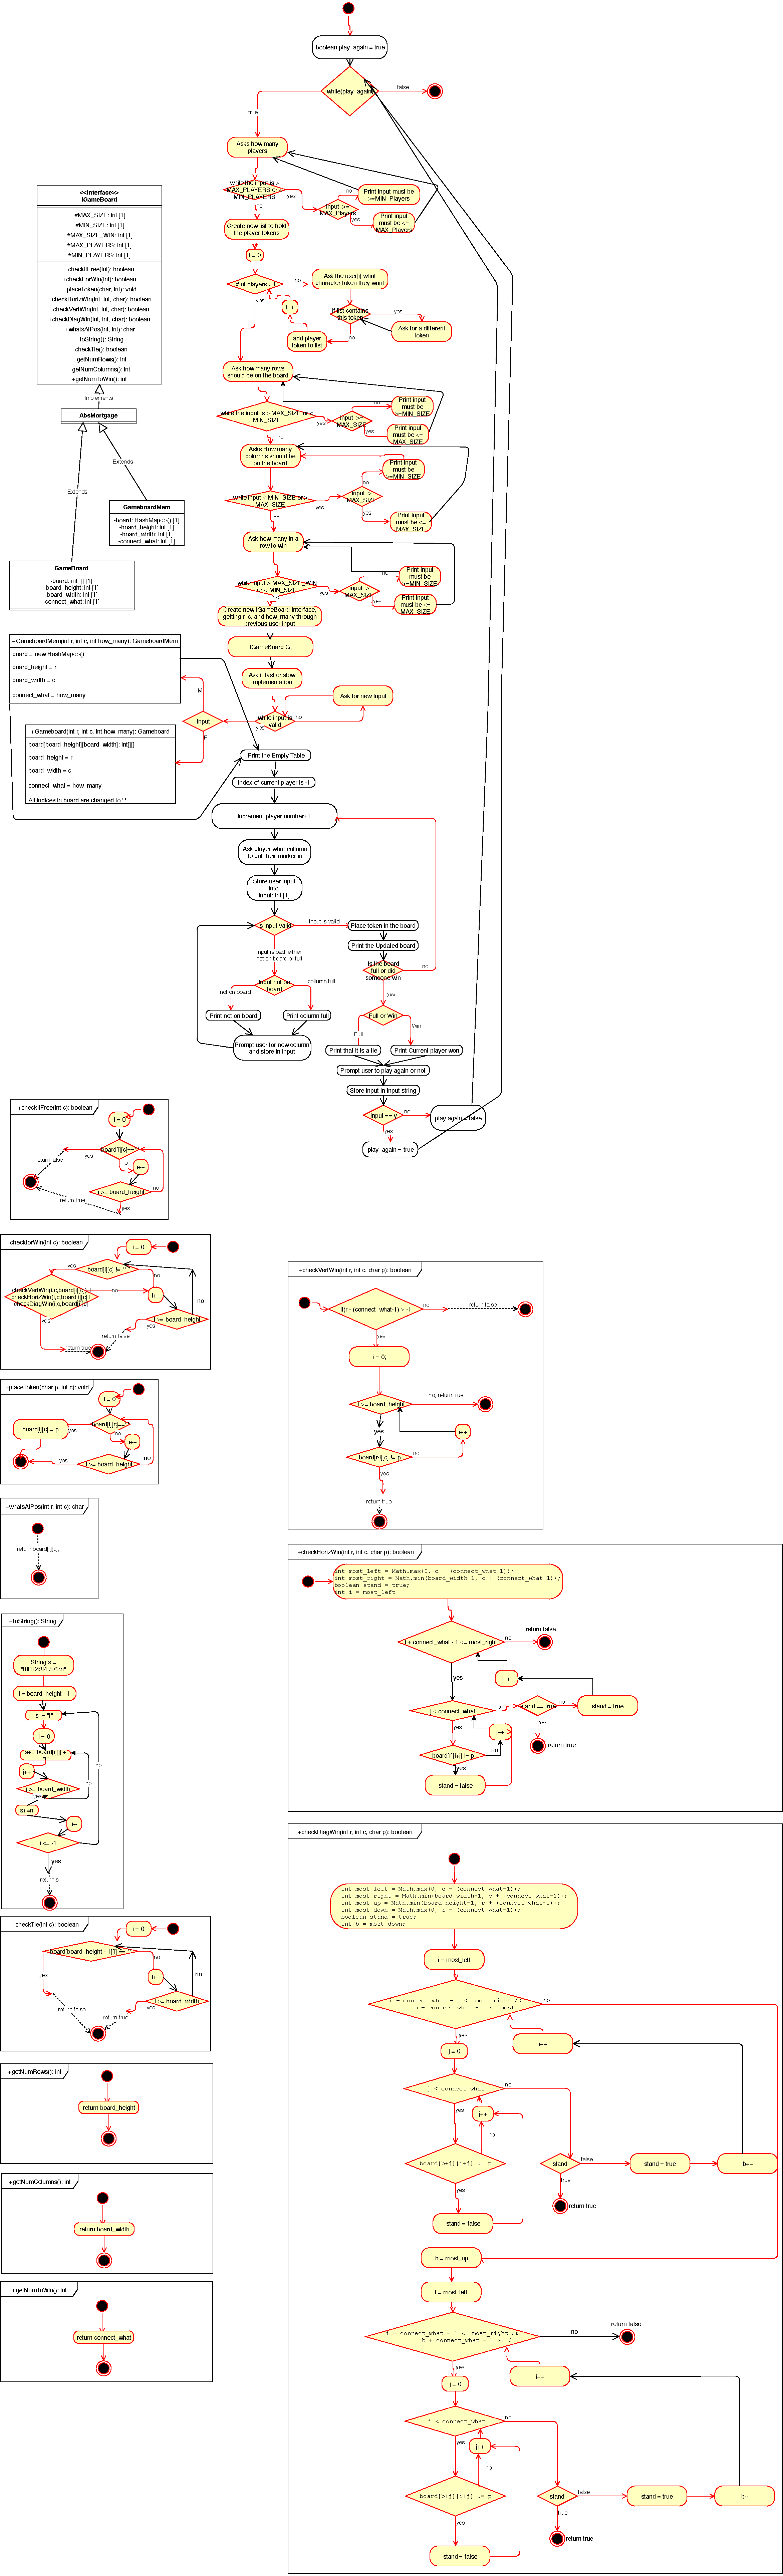
\includepdf[pages={1}]{2150HW2}
\section{Deployment}
\paragraph{}
Navigate inside the directory cpsc2150 

Enter the command \texttt make

Enter the command \texttt make run
\end{document}

